\section{Magnetisches Feld}
\subsection{Moodle-Übung}
\begin{enumerate}
  \item Magnetische Kräfte zwischen drei/zwei parallel verlaufenden, stromdurchflossenen geraden Leitern, wobei $a >> d$
        \begin{figure}[h!]
          \begin{center}
            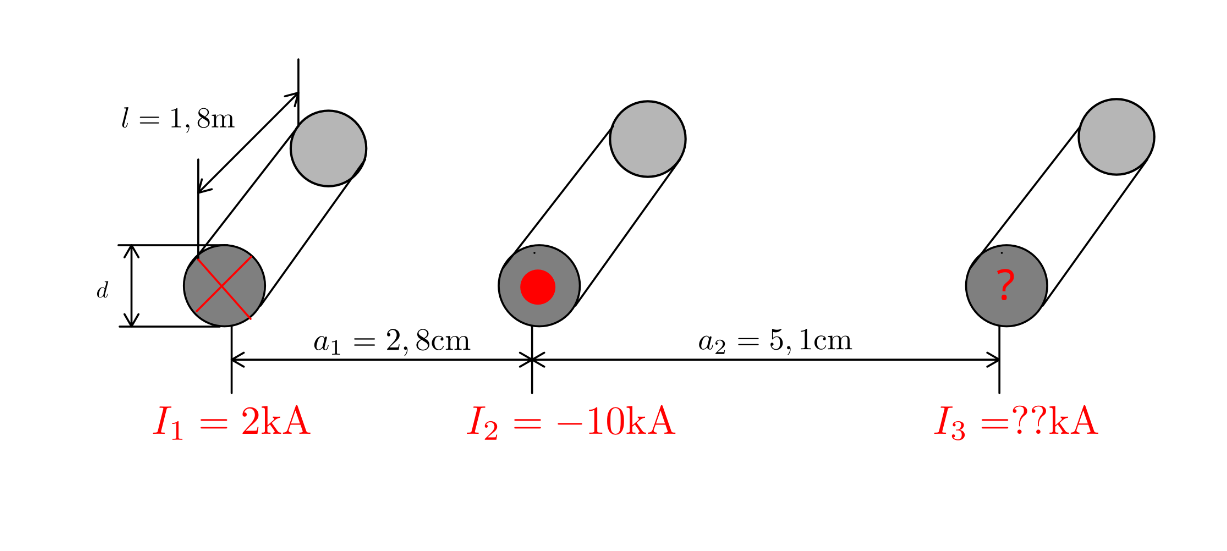
\includegraphics[width=0.75\textwidth]{img/Magnetisches-Feld/A1.png}
          \end{center}
          \caption{Moodle-Übung magnetisches Feld – Kraftwirkung auf drei Leitern}
        \end{figure}

        \begin{align*}
          F_{12}             & = \frac{\mu}{2\pi}\cdot \frac{I_1\cdot I_2}{a}\cdot l                                 \\
          \text{Für } F_{12} & = F_{32} \text{ dann gilt:}                                                           \\
          I_3                & = \frac{I_1\cdot a_2}{a_1}                                                            \\
                             & = \frac{2\cdot 10^{3}\text{A}\cdot 5,1\cdot 10^{-2}\text{m}}{2,8\cdot 10^{3}\text{m}} \\
                             & = 3,64\text{kA}                                                                       \\                                                                   \\
        \end{align*}

        \begin{align*}
          F_{31} & =\frac{\mu\cdot\mu_{0}}{2\pi}\cdot\frac{I_{1}\cdot I_{3}}{a}\cdot l                                                                                                                         \\
                 & =\frac{4\pi\cdot 10^{-7}\frac{\text{H}}{\text{m}}}{2\pi}\cdot\frac{2\cdot 10^{3}\text{A}\cdot 3,64\cdot 10^{3}\text{A}}{2,8\cdot 10^{-2}\text{m}+5,1\cdot 10^{-2}\text{m}}\cdot 1,8\text{m} \\
                 & = 33,202\text{N}                                                                                                                                                                            \\
                 & \Rightarrow |33,20\text{N}|                                                                                                                                                                 \\                                                                                                                                                                 \\
        \end{align*}

        \begin{align*}
          F_{21} & =\frac{\mu\cdot\mu_{0}}{2\pi}\cdot\frac{I_{2}\cdot I_{1}}{a}\cdot l                                                                                               \\
                 & =\frac{4\pi\cdot 10^{-7}\frac{\text{H}}{\text{m}}}{2\pi}\cdot\frac{2\cdot 10^{3}\text{A}\cdot(-10\cdot 10^{3}\text{A})}{2,8\cdot 10^{3}\text{m}}\cdot 1,8\text{m} \\
                 & =-257,14\text{N}                                                                                                                                                  \\
                 & \Rightarrow |257,14\text{N}|                                                                                                                                      \\                                                                                                                                                              \\
        \end{align*}

        \begin{align*}
          F_{1} & = F_{21}+F_{31}                   \\
                & =-257,14\text{N} + 33,202\text{N} \\
                & = -223,94\text{N}                 \\
                & \Rightarrow |223,94\text{N}|      \\                                                                                                                                                              \\
        \end{align*}

  \item Magnetische Kräfte, die zwischen drei räumlich verteilten, stromdurchflossenen Leitern liegen, wobei  $a>> d$


        \begin{figure}[h!]
          \begin{center}
            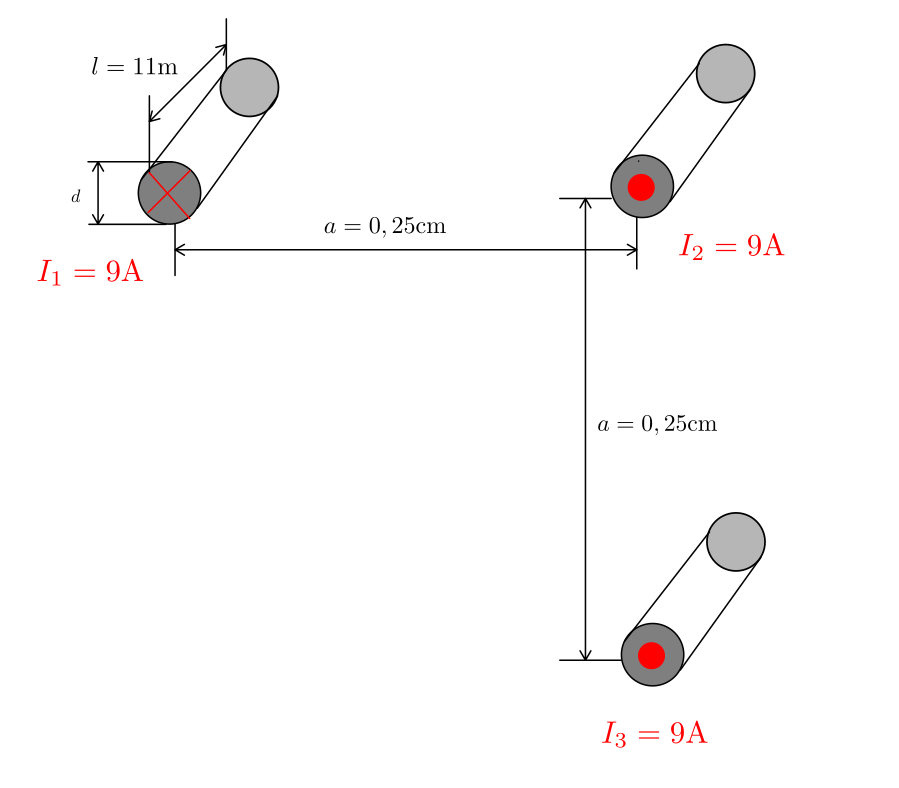
\includegraphics[width=0.6\textwidth]{img/Magnetisches-Feld/A2.png}
          \end{center}
          \caption{Moodle-Übung magnetisches Feld – Kraftwirkung auf drei Leitern}
        \end{figure}

        \begin{align*}
          F_{13} & =\frac{\mu\cdot\mu_{0}}{2\pi}\cdot\frac{I_{1}\cdot I_{3}}{a}\cdot l                                                                     \\
                 & =\frac{4\pi\cdot 10^{-7}\frac{\text{H}}{\text{m}}}{2\pi}\cdot\frac{9\text{A}\cdot 9\text{A}}{0,25\text{m}\cdot\sqrt{2}}\cdot 11\text{m} \\
                 & = 0,713\cdot 10^{-3}\text{N}                                                                                                            \\
                 & \Rightarrow |0,713\cdot 10^{-3}|                                                                                                        \\
          \\
          \text{Hinweis:}                                                                                                                                  \\
                 & a=\sqrt{a^2+a^2}                                                                                                                        \\
                 & =\sqrt{2\cdot a^2}                                                                                                                      \\
                 & = a\cdot\sqrt{2}                                                                                                                        \\                                                                                       \\
        \end{align*}

        \begin{figure}[!h]
          \begin{center}
            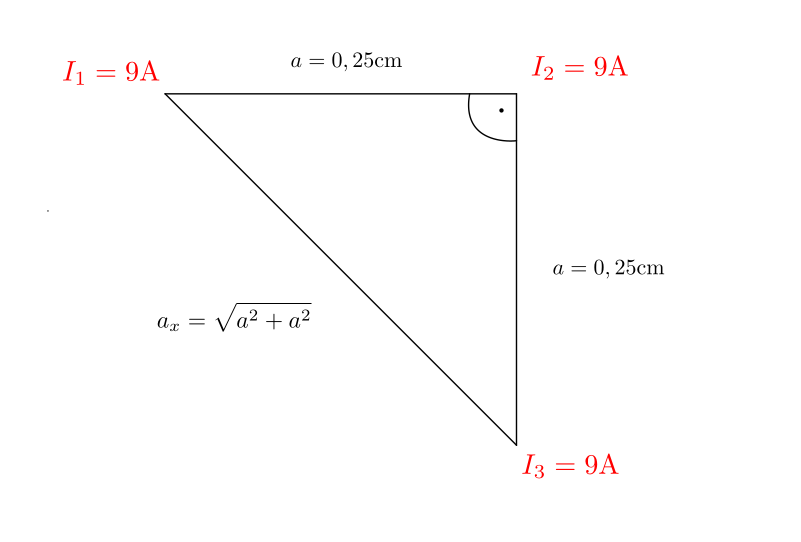
\includegraphics[width=0.6\textwidth]{img/Magnetisches-Feld/A2.1.png}
          \end{center}
          \caption{Moodle-Übung magnetisches Feld – Aufgelöste Darstellung der Anordnung}
        \end{figure}
        \newpage

        \begin{align*}
          F_{23} & =\frac{\mu\cdot\mu_{0}}{2\pi}\cdot\frac{I_{2}\cdot I_{3}}{a}\cdot l                                                           \\
                 & =\frac{4\pi\cdot 10^{-7}\frac{\text{H}}{\text{m}}}{2\pi}\cdot\frac{9\text{A}\cdot (-9\text{A})}{0,25\text{m}}\cdot 11\text{m} \\
                 & = -0,504\cdot 10^{-3}\text{N}                                                                                                 \\
                 & \Rightarrow |0,504\cdot 10^{-3}\text{N}|                                                                                      \\                                                                                                                                                                 \\
        \end{align*}

        Um die gesamte Kraft auf den Leiter drei zu ermitteln, müssen die auf den Leiter drei wirkenden Kräfte in X und Y Komponenten zerlegt werden.

        \begin{figure}[h!]
          \begin{center}
            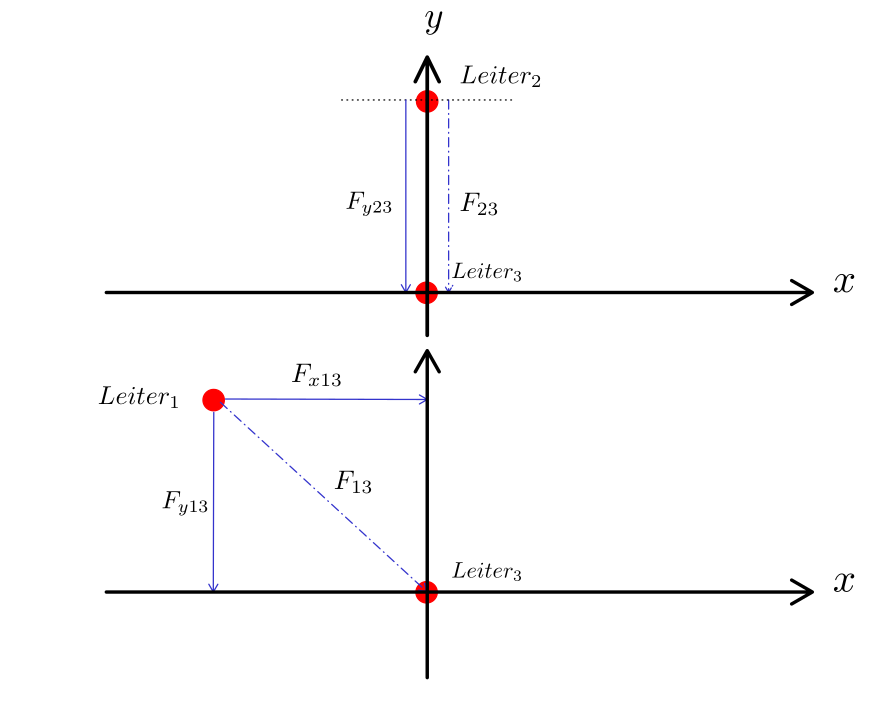
\includegraphics[width=0.75\textwidth]{img/Magnetisches-Feld/A2.2.1.png}
          \end{center}
          \caption{Moodle-Übung magnetisches Feld – Aufgelöste Darstellung der Anordnung, für die Kräftezerlegung}
        \end{figure}

        \begin{table}[h!]
          \centering
          \begin{tabular}{llll}
            \hline
            sin & cos & tan & ctan \\ \hline
            G   & A   & G   & A    \\
            H   & H   & A   & G    \\ \hline
          \end{tabular}
        \end{table}


        \begin{align*}
          F_{3y} & = F_{y23}\cdot\sin{\varphi}+F_{y13}\sin{\varphi}                                                  \\
                 & =  -0,504\cdot 10^{-3}\text{N}\cdot\sin{90^\circ}+(0,713\cdot 10^{-3}\text{N}\cdot\sin{45^\circ}) \\
                 & = 167,135 10^{-3}\text{N}                                                                         \\                                                                                                                                                                 \\
        \end{align*}

        \begin{align*}
          F_{3x} & = F_{x23}\cdot\sin{\varphi}+F_{x13}\sin{\varphi}                                                  \\
                 & =  0,713\cdot 10^{-3}\text{N}\cdot\cos{45^\circ}+(-0,504\cdot 10^{-3}\text{N}\cdot\cos{90^\circ}) \\
                 & = 0,504 10^{-3}\text{N}                                                                           \\                                                                                                                                                                 \\
        \end{align*}

\end{enumerate}
